% !TeX spellcheck = ru_RU
% !TEX root = bfs_lodygin.tex

\section{Эксперимент}

В данном разделе предлагается рассмотреть результаты экспериментального исследования реализованного алгоритма обхода графа в ширину. Основная задача: выявить зависимость производительности алгоритма от входных параметров графа и количества асинхронных потоков, обрабатывающих данный алгоритм.

\subsection{Условия эксперимента}
Для экспериментов использовалась рабочая станция с процессором Intel Core i5-10300H с тактовой частотой 2.50GHz, RAM DDR4 объемом 8гб под управлением OC Windows 10 Pro версии 21H2.

\subsection{Исследовательские вопросы }

\begin{itemize}
\item[\textbf{RQ1:}] При каких параметрах графа выгоднее использовать параллельную версию алгоритма, а при каких последовательную?
\item[\textbf{RQ2:}] Использование какого количества потоков даёт наибольший выигрыш в производительности и почему?
\end{itemize}


\subsection{Метрики}
В качестве метрик производительности используется время, требуемое на завершение алгоритма. Показатели времени получены с помощью библиотеки \texttt{BenchmarkDotNet v0.13.5}\footnote{\url{https://github.com/dotnet/BenchmarkDotNet} (дата доступа:   \DTMdate{2023-05-21}).}.

Для анализа алгоритма было решено воспользоваться собственным генератором графов нужного размера с нужной плотностью. Данный подход позволяет минимизировать влияние разницы прочих параметров на исследуемый, следовательно результаты, полученные в таком исследовании, позволят точнее выявить необходимые зависимости, нежели при подборе базы графов из реальных существующих. Генератор принимает на вход количество вершин в графе и параметр \texttt{density} типа \texttt{float}, отвечающий за плотность графа. По заданным вершинам создается двумерный массив, заполненный либо \texttt{Option.None}, если плотность графа менее $50\%$, либо случайным числом типа \texttt{int}, обёрнутым в тип \texttt{Option}. По параметру плотности графа вычисляется количество рёбер, необходимое для достижения такой плотности.
Затем, запускается цикл, в котором генерируются два числа от нуля до количества вершин и, в зависимости от того, является граф плотным или нет, ячейки массива, соответствующие сгенерированным числам, заполняются либо случайными числами типа \texttt{int}, обёрнутым в тип \texttt{Option}, либо \texttt{Option.None}.  


\subsection{Результаты}

Входные параметры:
 \begin{enumerate}
 \item  \texttt{Vertices} --- количество вершин в графе; 
 \item  \texttt{Density} --- плотность графа;
 \item \texttt{parallelMult} --- уровень распараллеливания функции умножения, каждый уровень увеличивает число подзадач в 4 раза;
  \item \texttt{parallelAdd} --- уровень распараллеливания функции сложения, каждый уровень увеличивает число подзадач в 2 раза.
\end{enumerate}

Результаты замеров:
\begin{enumerate}
\item  \texttt{Time} --- результат измерений в мс ( за исключением таблицы~\ref{bfscomparison}, где вермя измерений указано в микросекундах и таблицы~\ref{bfsmaxgraph}, где время указано в секундах);
\end{enumerate}

Замеры проводились начиная от сравнительно малых графов (500 вершин), заканчивая графами с 5000 вершинами. Выбор максимального размера графа связан с ограничением оперативной памяти системы, на которой производились вычисления.

В таблице~\ref{bfs0} представлены результаты замеров времени работы последовательного алгоритма при различных входных параметрах графа. Из данной таблицы видно, что время работы алгоритма возрастает с увеличением плотности графа, а затем, когда граф достигает плотности $0.7$ начинает снижаться. Не трудно догадаться, что при высокой плотности графа уменьшается количество шагов алгоритма, необходимых для его завершения, так как за каждый шаг будет осуществляться переход в большее количество смежных вершин, следовательно общее время работы уменьшается.

\begin{table}[h]
\centering
    \caption{Производительность последовательного алгоритма обхода графов в ширину.}
    \rowcolors{2}{black!2}{black!10}
    \scalebox{0.7}{
    \begin{tabular}{| a | r | r | a | r | r |}
    \hline
        \textsc{Vertices} & \textsc{Density} & \textsc{Time} &
         \textsc{Vertices} & \textsc{Density} & \textsc{Time} \\ 
        \hline
        500 & 0.1 & $17 \pm 0.06$ & 2500 & 0.1 & $429 \pm 2$  \\ 
        500 & 0.3 & $33 \pm 0.3$ & 2500 & 0.3 & $860 \pm 3$ \\ 
        500 & 0.7 & $42 \pm 0.2$ & 2500 & 0.7 & $1095 \pm 3$  \\ 
        500 & 0.9 & $36 \pm 0.17$ & 2500 & 0.9 & $980 \pm 4$  \\ 
        
        1000 & 0.1 & $68 \pm 0.4$ & 5000 & 0.1 & $1717 \pm 3$ \\ 
        1000 & 0.3 & $137 \pm 0.6$ & 5000 & 0.3 & $3531 \pm 20$ \\ 
        1000 & 0.7 & $179 \pm 1.2$ & 5000 & 0.7 & $4421 \pm 9$ \\ 
        1000 & 0.9 & $158 \pm 0.3$ & 5000 & 0.9 & $3984 \pm 14$ \\ 
    \hline    
    \end{tabular}%
    }
    \label{bfs0}
\end{table}

В таблице~\ref{bfsparallel} приведены результаты замеров времени работы параллельного алгоритма обхода графа при различных параметрах. Для удобства, при каждом параметре плотности графа взята наилучшая скорость среди всех параллельных версий алгоритма. Из полученных результатов можно заметить, что при увеличении размеров графа, наиболее оптимальное количество подзадач для параллельных вычислений выравнивается к 16 для функции умножения. Стоить отметить, что на достаточно больших графах, при одном и том же уровне распараллеливания функции умножения, влияние распараллеливания функции сложения становится не столь существенным, любая из комбинаций даёт один и тот же результат по времени в пределах погрешности. Связано это с тем, что наибольший процент времени выделяется под функцию умножения, как наиболее затратную по ресурсам.

\begin{table}[H]
\centering
    \caption{Производительность параллельного алгоритма обхода графов в ширину (лучшие данные по метрике). Графа \texttt{SpeedUp} показывает отношение скорости работы параллельной версии алгоритма к скорости работы последовательной версии. }
    \rowcolors{2}{black!2}{black!10}
    \scalebox{0.5}{
    \begin{tabular}{| a | r | r | r | r | r |}
    \hline
        \textsc{Vertices} & \textsc{Density} & \textsc{parallelMult} & \textsc{parallelAdd} & \textsc{Time} & \textsc{SpeedUp}\\
        \hline
        500 & 0.1 & 2 & 1 & $9 \pm 0.2$ & 0.53\\ 
        500 & 0.3 & 1 & 1 & $19 \pm 0.2$ & 0.57\\ 
        500 & 0.7 & 1 & 2 & $26 \pm 0.2$ & 0.62\\
        500 & 0.9 & 2 & 2 & $23 \pm 0.3$ & 0.64\\        
        1000 & 0.1 & 1 & 1 & $37 \pm 0.7$ & 0.54\\ 
        1000 & 0.3 & 1 & 1 & $73 \pm 0.9$ & 0.53\\ 
        1000 & 0.7 & 1 & 2 & $99 \pm 1.4$ & 0.55\\ 
        1000 & 0.9 & 1 & 3 & $91 \pm 1.5$ & 0.57\\ 
        2500 & 0.1 & 2 & 3 & $241 \pm 5$ & 0.56 \\
        2500 & 0.3 & 2 & 3 & $464 \pm 9$ & 0.54 \\
        2500 & 0.7 & 2 & 3 & $650 \pm 11$ & 0.59\\
        2500 & 0.9 & 2 & 1 & $585 \pm 12$ & 0.6  \\ 
        5000 & 0.1 & 2 & 1 & $970 \pm 19$ & 0.56 \\ 
        5000 & 0.3 & 2 & 3 & $1814 \pm 36$ & 0.51 \\
        5000 & 0.7 & 2 & 3 & $2606 \pm 51$ & 0.59 \\ 
        5000 & 0.9 & 2 & 1 & $2326 \pm 45$ & 0.58 \\ 
    \hline    
    \end{tabular}%
    }
    \label{bfsparallel}
\end{table}

Для более точного анализа были произведены дополнительные замеры при очень малых размерах входного графа (таблица~\ref{bfscomparison}). Выяснилось, что при малых размерах графа последовательная версия работает значительно быстрее, чем параллельная.

\begin{table}[h]
\centering
    \caption{Сравнение производительности параллельного и обычного Bfs на графах с малым количеством вершин. Графа \texttt{SpeedUp} показывает отношение скорости работы параллельной версии алгоритма к скорости работы последовательной версии.}
    \rowcolors{2}{black!2}{black!10}
    \scalebox{0.7}{
    \begin{tabular}{| a | r | r | r | r |}
    \hline
        \textsc{Vertices} & \textsc{Density} & \textsc{TimeBfs} & \textsc{TimeParallelBfs} & \textsc{SpeedUp}\\
        \hline
        10 & 0.1 & $15 \pm 0.03$ & $53 \pm 0.2$ & 3.5 \\ 
        10 & 0.3 & $20 \pm 0.4$ & $78 \pm 0.3$ & 3.9 \\ 
        10 & 0.7 & $27 \pm 0.5$ & $60 \pm 0.4$ & 2.2 \\
        10 & 0.9 & $25 \pm 0.6$ & $44 \pm 0.4$ & 1.76\\ 
    \hline    
    \end{tabular}%
    }
    \label{bfscomparison}
\end{table}

Аналогично, чтобы исследовать оптимальное разделение на подзадачи для функции умножения, были проведены замеры с теми же размерами и плотностями графа, но с использованием последовательной функции сложения. Результаты приведены в таблице~\ref{bfsparallelmult}.

\begin{table}[h]
\centering
    \caption{Производительность параллельного алгоритма обхода графов в ширину с использованием последовательной функции сложения веторов.}
    \rowcolors{2}{black!2}{black!10}
    \scalebox{0.6}{
    \begin{tabular}{| a | r | r | r | a | r | r | r |}
    \hline
        \textsc{Vertices} & \textsc{Density} & \textsc{parallelMult} & \textsc{Time} &
        \textsc{Vertices} & \textsc{Density} & \textsc{parallelMult} & \textsc{Time} \\ 
        \hline
        500 & 0.1 & 1 & $9,8 \pm 0.1$ & 2500 & 0.1 & 2 & $240 \pm 3$  \\ 
        500 & 0.3 & 1 & $19 \pm 0.4$ & 2500 & 0.3 & 2 & $470 \pm 9$ \\ 
        500 & 0.7 & 1 & $26 \pm 0.5$ & 2500 & 0.7 & 2 & $661 \pm 13$  \\
        500 & 0.9 & 2 & $24 \pm 0.4$ & 2500 & 0.9 & 2 & $620 \pm 12$  \\ 
        
        1000 & 0.1 & 1 & $36 \pm 0.5$ & 5000 & 0.1 & 2 & $923 \pm 18$ \\
        1000 & 0.3  & 1 & $72 \pm 1.4$ & 5000 & 0.3 & 2 & $1843 \pm 36$ \\ 
        1000 & 0.7 & 1 & $98 \pm 1.6$ & 5000 & 0.7 & 2 & $2571 \pm 39$ \\ 
        1000 & 0.9 & 1 & $90 \pm 1.1$ & 5000 & 0.9 & 2 & $2372 \pm 41$ \\
    \hline    
    \end{tabular}%
    }
    \label{bfsparallelmult}
\end{table}

В ходе замеров было установлено, что при увеличении размеров графа, вне зависимости от плотности, время работы алгоритма при 16 подзадачах для функции умножения хоть и больше, чем при работе с 64 подзадачами, но разрыв становится все меньше и меньше. Вследствие этого наблюдения, было решено произвести замеры для параллельных версий алгоритма для графов гораздо большего размера, но маленькой плотности с целью выяснить, сможет ли версия с 64 подзадачами обогнать по производительности версию с 16 подзадачами. Результаты приведены в таблице~\ref{bfsmaxgraph}.

\begin{table}[h]
\centering
    \caption{Сравнение производительности алгоритма обхода в ширину при использовании 16 и 64 подзадач для функции умножения. Графа \texttt{SpeedUp} показывает отношение скорости работы алгоритма при 64 подзадачах к скорости работы при 16 подзадачах.}
    \rowcolors{2}{black!2}{black!10}
    \scalebox{0.6}{
    \begin{tabular}{| a | r | r | r | r | r |}
    \hline
        \textsc{Vertices} & \textsc{Density} & \textsc{parallelMult} & \textsc{Time} &
        \textsc{SpeedUp} \\ 
        \hline
        1000 & 0.1 & 2 & $0.04 \pm 0.0003$ & 1.25 \\
        2500 & 0.1 & 2 & $0.24 \pm 0.002$ & 1.22 \\ 
        5000 & 0.1 & 2 & $0.9 \pm 0.03$ & 1.2 \\
        10000 & 0.1 & 2 & $4 \pm 0.07$ & 1.25 \\ 
    \hline    
    \end{tabular}%
    }
    \label{bfsmaxgraph}
\end{table}

Однако, как показало дополнительное измерение при графе с 10000 вершинами, по производительности всё так же лидирует распараллеливание на 16 подзадач, причём разрыв между скоростями вырос.

Результаты, полученные с помощью \texttt{BenchmarkDotNet} были проверены на адекватность с помощью библиотек \texttt{SciPy v1.10.1}\footnote{\url{https://scipy.org/} (дата доступа:   \DTMdate{2023-05-21}).}, \texttt{NumPy v1.24.3}\footnote{\url{https://numpy.org/} (дата доступа:   \DTMdate{2023-05-21}).} и \texttt{Matplotlib v3.7.1}\footnote{\url{https://matplotlib.org/} (дата доступа:   \DTMdate{2023-05-21}).} на языке \texttt{Python}. Например, рассмотрим данные, полученные при измерении производительности параллельной версии алгоритма на графе с 5000 вершинами плотности $0.9$ и уровнями распараллеливания parallelMult, равным двум, и parallelAdd, равным 1. Результаты замеров приведены в таблице~\ref{data}. 

\begin{table}[h]
\centering
    \caption{Замеры времени работы параллельной версии алгоритма на графе с 5000 вершинами плотности $0.9$. Функция умножения разделена на 16 подзадач, функция сложения на две. Время измерено в секундах.}
    \rowcolors{2}{black!2}{black!10}
    \scalebox{0.6}{
    \begin{tabular}{| a | r | r | r | r | r | r | r | r | r | r |}
    \hline
    N & 1 & 2 & 3 & 4 & 5 & 6 & 7 & 8 & 9 & 10 \\
    \hline
    Time & 2.4081 & 2.3506 & 2.3857 & 2.3383 & 2.2634 & 2.2931 & 2.2984 & 2.3895 & 2.2800 & 2.2899\\
    N & 11 & 12 & 13 & 14 & 15 & 16 & 17 & 18 & 19 & 20\\
    \hline
    Time & 2.3293 & 2.2977 & 2.2358 & 2.3113 & 2.4044 & 2.3317 & 2.3054 & 2.2614 & 2.4011 & 2.3421 \\
    \hline    
    \end{tabular}%
    }
    \label{data}
\end{table}

С помощью функций \texttt{scipy.stats.shapiro()} (тест Шапиро-Уилка) и \texttt{scipy.stats.normaltest()} (критерий согласия Пирсона) было проверено соответствие выборки нормальному распределению. Значение \texttt{pvalue} в результате проверок равнялось 0.36 (Шапиро) и 0.5 (Пирсон), что позволяет нам не отклонять \enquote{нулевую гипотезу} и считать полученные данные как нормальное распределение. Далее, с помощью функций \texttt{np.mean()} и \texttt{np.std()} были посчитаны среднее значение $Mean = 2.32586$ и стандартное отклонение $StdDev = 0.051$. Аналогичные результаты были получены и библиотекой \texttt{BenchmarkDotNet}: $Mean = 2.326$, $StdDev = 0.051$. При помощи \texttt{matplotlib.pyplot.hist()} была построена гистограмма (рисунок~\ref{fig:plot}) из полученной выборки.

\begin{figure}[H]
    \centering
    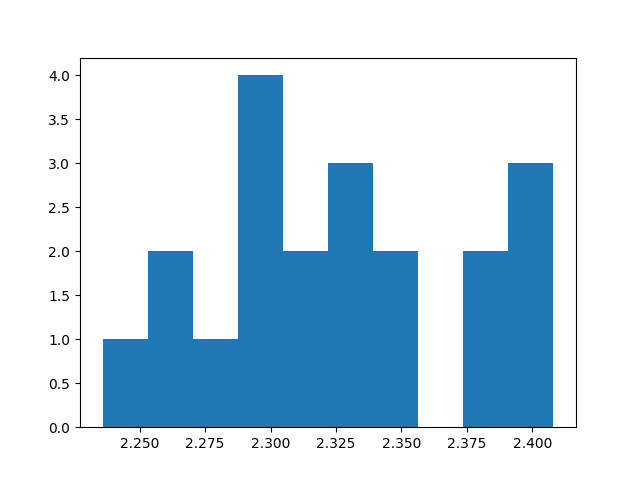
\includegraphics[width=\textwidth]{figures/plot.png}
    \caption{Гистограмма распределения данных}
    \label{fig:plot}
\end{figure}

\subsubsection{RQ1} Исходя из полученных данных, последовательная версия алгоритма работает быстрее параллельной только на очень малых графах, когда накладные расходы на выделение дополнительных потоков и их синхронизацию влияют сильнее, чем ускорение относительно последовательной версии. При входных графах от 100 вершин и более, параллельная версия даёт внушительный прирост к производительности при любых параметрах плотности.
\subsubsection{RQ2} В ходе экспериментов было установлено, что использование разделения на 16 подзадач, начиная с определённых размеров графа (2500 вершин для системы, используемой при замерах), даёт максимальный прирост по производительности алгоритма обхода в ширину. Такой результат можно объяснить количеством ядер процессора. Система, на которой производились замеры имеет 4-х ядерный процессор \texttt{Intel Core i5-10300H}, вследствие чего количество независимых вычислителей равняется четырём. С другой стороны, данный процессор поддерживает технологию \texttt{Hyper-Threading}, позволяющую разделить одно ядро процессора на 2 отдельных логических процессора, работающих независимо. Таким образом наилучшая производительность наблюдается на 8 потоках, каждый из которых обрабатывает по 2 подзадачи. Польза от такого разделения влияет на конечное время работы алгоритма сильнее, чем затраты времени на выделение необходимых потоков и синхронизацию их работы.